\documentclass[twocolumn, dvipdfmx,12pt]{beamer}
\usepackage{bxdpx-beamer}
\usepackage{pxjahyper}
\usepackage{tikz}
\usepackage{here}
\usepackage{graphicx}
\renewcommand{\kanjifamilydefault}{\gtdefault}

\usepackage{amsmath}
\usepackage{amsfonts}
\usepackage{amssymb}
\usepackage{color}
\usepackage{tcolorbox}
\usepackage{forest}
\usepackage{ascmac}
\usepackage{fancybox}
\usepackage{eclbkbox}
\usepackage{multicol}
\usepackage{xcolor}
\usetikzlibrary{arrows.meta}
\usetikzlibrary{positioning}
\usetikzlibrary{decorations.pathreplacing,calligraphy}
\usetikzlibrary{patterns}
\usetheme{metropolis}  

\setlength{\columnsep}{1.5cm}
\setlength{\columnseprule}{0.2pt}

% blockのスタイルをカスタマイズ
\setbeamercolor{block title}{bg=blue!30,fg=black} % タイトルの背景色とテキストの色
\setbeamercolor{block body}{bg=blue!10,fg=black} % ボディの背景色とテキストの色

\usepackage[usetype1]{uline--}

\title{第3回MPC勉強会}
\author{鶴原康太}

\begin{document}

    \frame{\maketitle}

    \begin{frame}{今回の目標}
        \begin{equation*}
            -\frac{\partial V}{\partial t}\left(x,t\right) = \min _u H\left(x, u, \left( \frac{\partial V}{\partial x} \right)^T\left(x, t\right), t \right)
        \end{equation*}
    \end{frame}

    \begin{frame}{現在位置}
        \begin{columns}
            \begin{column}{.4\textwidth}
                \begin{enumerate}
                    \item \colorbox{yellow}{復習}
                    \item 動的計画法
                    \item HJB方程式
                    \item 最小原理
                    \item NMPC導入
                \end{enumerate}
            \end{column}
    
            \begin{column}{.6\textwidth}
                今までの内容覚えてますか?\\
                復習しましょう!!
            \end{column}
        \end{columns}
    \end{frame}

    \begin{frame}{最適制御とは}
        \begin{screen}
            状態方程式 \quad $\dot{x}(t) = f(x(t), u(t), t)$ \\
            評価関数 \qquad $J =$ 
            \tikz[remember picture, baseline=(T1.base)]{
                \node [fill=orange!20!white, inner sep=0pt, outer sep=0, minimum height=4ex] (T1) {$\varphi(x(t_f))$};
            }
            $+$
            \tikz[remember picture, baseline=(T2.base)]{
                \node [fill=red!20!white, inner sep=0pt, outer sep=0, minimum height=4ex] (T2) {$\int_{t_0}^{t_f} L(x(t), u(t), t) \, dt$}
            }
             
            \begin{tikzpicture}[remember picture, overlay]
              \node [below=0pt of T1, text=orange!80!black] {終端コスト};
              \node [below=0pt of T2, text=red!80!black] {ステージコスト};
            \end{tikzpicture}
        \end{screen}
        \centering{
            \begin{tikzpicture}
                \draw[->, >=stealth, semithick](-0.5, 0)--(7.5, 0)node[right]{$t$};
                \draw[->, >=stealth, semithick](0, -0.5)--(0, 3.5)node[above]{$x$};
                \draw[dashed](1.5, -0.5)node[below]{$t_0$}--(1.5, 3.5);
                \draw[dashed](6.0, -0.5)node[below]{$t_f$}--(6.0, 3.5);

                \footnotesize{
                    \fill[black](1.5, 1.5)circle(0.1)node[left]{$(t_0, x_0)$};
                    \fill[black](6.0, 2.5)circle(0.1)node[right]{$(t_f, x_f)$};
                }
                \draw[thick, black](1.5, 1.5)to[out=30, in=170](6.0, 2.5);
                \draw[thick, dashed, black](1.5, 1.5)to[out=50, in=150](6.0, 2.5);
                \draw[thick, dashed, black](1.5, 1.5)to[out=10, in=205](6.0, 2.5);

                \large{
                    \draw(3.7, 3.3)node{?};
                }
            \end{tikzpicture}
        }

        \footnotesize
    
    \end{frame}

    \begin{frame}{変分法1}
        \footnotesize
        \begin{screen}
            \begin{center}
                評価関数 \quad $J =\varphi(x(t_f))+\int_{t_0}^{t_f} L(x(t), u(t), t) \, dt$
            \end{center}
        \end{screen}
        \begin{tikzpicture}        
            \draw[->,>=stealth,semithick](-0.5,0)--(3.5,0)node[above]{$x$};
            \draw[->,>=stealth,semithick](0,-0.5)--(0,3.5)node[right]{$y$};
            \draw[very thick,domain=-1.7:1.7]plot(\x+1.5,\x*\x+0.5);
            \fill[red](1.5, 0.5)circle(0.1);
           
            \draw[->, red, very thick] (1.3, 0.75) to [out=150, in=-70] (0.75, 1.4);
            \draw[->, red, very thick] (1.7, 0.75) to [out=30, in=250] (2.25, 1.4);

            \draw[->,>=stealth,semithick](5.5,0)--(9.5,0)node[above]{$x$};
            \draw[->,>=stealth,semithick](6,-0.5)--(6,3.5)node[right]{$y$};

            \draw[dashed, blue, very thick, domain=-0.5:3.5]plot(\x+6,{0.4*cos(3 * \x r)+0.3*sin(6*\x r)+1.7});
            \draw[dashed, red, very thick, domain=-0.5:3.5]plot(\x+6,{0.3*cos(3 * \x r)+0.4*sin(6*\x r)+0.3*sin(8*\x r)+1.7});
            \draw[black, very thick, domain=-0.5:3.5]plot(\x+6,{0.2*cos(3 * \x r)+0.1*sin(6*\x r)+1.7});

            \fill[white](0, 4)node[black]{微分法}circle(0.1);
            \fill[white](6, 4)node[black]{変分法}circle(0.1);

            \fill[white](0.6, -1)node[black, right]{関数の勾配}circle(0.1);
            \fill[white](5.5, -1)node[black, right]{汎関数(関数の関数)の勾配}circle(0.1);

        \end{tikzpicture}

        \vspace{-0.8em}

        \begin{center}
            \colorbox{yellow}{評価関数$J$は関数$x(t)$,$u(t)$の関数なので汎関数とみなせる}
        \end{center}

    \end{frame}

    \begin{frame}{変分法2}
        \fontsize{7.8pt}{7.8pt}\selectfont


        \begin{multicols}{2}
            \colorbox{yellow}{評価関数$J$のみの停留条件}\\
                
            \vspace{1em}

            曲線の形状など入力を必要としない最適化に用いる

            \begin{equation*}
                J =\varphi(x(t_f))+\int_{t_0}^{t_f} L(x(t), \textcolor{red}{\dot{x}(t)}, t) \, dt
            \end{equation*}
            \begin{align*}
                \frac{\partial L}{\partial x} - \frac{d}{dt} \left( \frac{\partial L}{\partial \dot{x}} \right) = 0
            \end{align*}
            この等式が成立するのは始点と終点を初期値として与えられた場合である\\
            (2点境界値問題)\\
            
            \columnbreak

            \colorbox{yellow}{評価関数Jと状態方程式を考慮した停留条件}\\
            \vspace{1em}
            最適制御では入力を求めるのでこちらを用いる
            \begin{equation*}
                J =\varphi(x(t_f))+\int_{t_0}^{t_f} L(x(t), \textcolor{red}{u(t)}, t) \, dt
            \end{equation*}

            \begin{align*}
                \begin{cases}
                    &x(t_0)=x_0 \\
                    &\lambda(t_f)=\left(\frac{\partial \varphi}{\partial x}\right)^\top \\
                    &\frac{d\lambda}{dt}=-\left(\frac{\partial H}{\partial x}\right)^\top\\
                    &\frac{dx}{dt}=f(x,u,t)=\left(\frac{\partial H}{\partial \lambda}\right)^\top \\
                    &\frac{\partial H}{\partial u}=0 \\
                \end{cases}
            \end{align*}
                このとき$H=L+\lambda ^\top f + \rho ^\top C$と拡張すれば入力制約も考慮できる
        \end{multicols}
                 
    \end{frame}

    \begin{frame}{変分法3}
        \fontsize{9.5pt}{9.5pt}\selectfont

        Q.\quad なぜ異なる形のEuler-Lagrange方程式があるの? \\
        A.\quad 変分問題の停留条件の式の総称がEuler-Lagrange方程式\\
                \qquad 決まった式の形ではない.\\

        \vspace{1em}
        Q.\quad 最適制御のEuler-Lagrange方程式は入力制約がある場合は使えないの?\\
        A.\quad 使える.
    \end{frame}
    \begin{frame}{第1回、第2回まとめ}
        \begin{itembox}[l]{第1回}
            評価関数を予め,時間的に離散化することによって最適化問題に落とし込んだ
        \end{itembox}
        \begin{itembox}[l]{第2回}
            評価関数を汎関数と考え,変分法を利用して最適制御が満たすEuler-Lagrange方程式を導いた
        \end{itembox}
    \end{frame}

    \begin{frame}{最適性条件まとめ}
        \fontsize{6.5pt}{6.5pt}\selectfont
        
        \begin{columns}
            \begin{column}{.6\textwidth}
                \begin{itembox}[l]{時間を考慮しない}
                    \begin{itembox}[l]{線形MPC}
                        予め時間を考慮して出した式から出た最適化問題を解いたから
                        最適化問題自体は時間を考慮不要\\
                    \end{itembox}
                    \colorbox{yellow}{Lagrangeの未定乗数法}\\
                    \begin{align*}
                        &L(x, \lambda) = f(x) + \lambda^T g(x)\\
                        &\nabla L(x, \lambda)=0
                    \end{align*}
                    \colorbox{yellow}{KKT条件}\\
                    \begin{align*}
                        \nabla f(x^*) &+ \sum_{i=1}^m \lambda_i^* \nabla g_i(x^*) + \sum_{j=1}^n \mu_j^* \nabla h_j(x^*) = 0 \\
                        g_i(x^*) &\leq 0 \quad \text{for all } i \\
                        \lambda_i^* &\geq 0 \quad \text{for all } i \\
                        \lambda_i^* g_i(x^*) &= 0 \quad \text{for all } i \\
                        h_j(x^*) &= 0 \quad \text{for all } j
                    \end{align*}
                \end{itembox}
            \end{column}

            \begin{column}{.55\textwidth}
                \begin{itembox}[l]{時間を考慮}
                    \begin{itembox}[l]{非線形MPC}
                        時間で離散化せずに直接最適化問題を解きたい
                    \end{itembox}
                    \colorbox{yellow}{Euler-Lagrange方程式}\\
                    \begin{align*}
                        \begin{cases}
                            &x(t_0)=x_0 \\
                            &\lambda(t_f)=\left(\frac{\partial \varphi}{\partial x}\right)^\top \\
                            &\frac{d\lambda}{dt}=-\left(\frac{\partial H}{\partial x}\right)^\top\\
                            &\frac{dx}{dt}=f(x,u,t)=\left(\frac{\partial H}{\partial \lambda}\right)^\top \\
                            &\frac{\partial H}{\partial u}=0 \\
                        \end{cases}
                    \end{align*}
                    \begin{columns}
                        \begin{column}{.5\textwidth}
                            \begin{center}
                                \begin{itembox}[l]{動的計画法}
                                    \begin{tikzpicture}
                                        \draw[->](0, 0)node[above]{Bellman方程式}--(0, -0.5)node[below]{HJB方程式};
                                    \end{tikzpicture}
                                \end{itembox}
                            \end{center}
                        \end{column}
                        \begin{column}{.5\textwidth}
                            \begin{tikzpicture}
                                \draw(0, 0)node{最小原理}circle[radius=0.7];
                            \end{tikzpicture}
                        \end{column}
                    \end{columns}
                    
                \end{itembox}
            \end{column}
        \end{columns}
    \end{frame}

    \begin{frame}{最適化の多様な定式}
        \scriptsize
        Q.なぜ似たようなものがいくつもあるのか??\\

        A.\begin{itemize}
            \item 最適制御を異なる視点で考えている
            \item 解法精度が良ければ同じ結果に収束するが,問題によって各手法の計算時間が異なる
            \item 同時期(冷戦期)に2人の天才によって最適制御が定式化された
        \end{itemize}

        \vspace{5mm}

        \begin{columns}

            \begin{column}{0.5\textwidth}
                \begin{boxnote}
                    \begin{columns}
                        \begin{column}{.5\textwidth}
                            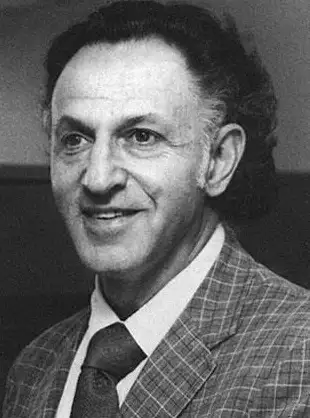
\includegraphics[clip, width = 2.0cm]{Bellman.png}\\
                            {\tiny Bellman}
                            \centering
                        \end{column}
                        \begin{column}{.5\textwidth}
                            アメリカ\\
                            \vspace{1em}
                            Bellman方程式 \\
                            HJB方程式 \\
                        \end{column}
                    \end{columns}
                \end{boxnote}
            \end{column}

            \begin{column}{0.5\textwidth}
                \begin{boxnote}
                    \begin{columns}
                        \begin{column}{.5\textwidth}
                            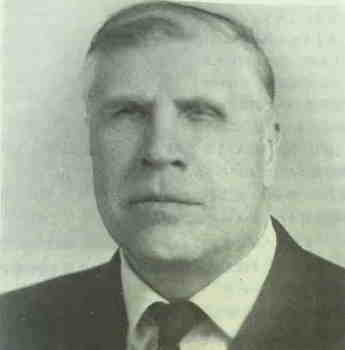
\includegraphics[clip, width = 2.0cm]{Pontryagin.png}\\
                            {\tiny Pontryagin}
                            \centering
                        \end{column}
                        \begin{column}{.5\textwidth}
                            ソ連\\
                            \vspace{2em}
                            最小原理 \\
                        \end{column}
                    \end{columns}
                \end{boxnote}
            \end{column}
        \end{columns}

    \end{frame}

    \begin{frame}{現在位置}
        \footnotesize
        \begin{columns}
            \begin{column}{.35\textwidth}
                \begin{enumerate}
                    \item 復習
                    \item \colorbox{yellow}{動的計画法}
                    \item HJB方程式
                    \item 最小原理
                    \item NMPC導入
                \end{enumerate}
            \end{column}
    
            \begin{column}{.7\textwidth}
                \fontsize{7.5pt}{3.5pt}\selectfont
                \begin{screen}
                    \begin{equation*}
                        V(x, t) = \min_{u[t, t+dt]} \left( L(x, u, t) dt + V \left( x + f(x, u, t) dt, t + dt \right) \right)
                    \end{equation*}
                \end{screen}
                \footnotesize
                方針:\\
                \qquad 問題を分割して最適制御を考える \\

            \end{column}
        \end{columns}
    \end{frame}

    \begin{frame}{動的計画法1}
        \footnotesize
        \begin{tcolorbox}[title=最適制御]
            状態方程式 \quad $\dot{x}(t) = f(x(t), u(t), t)$ \\
            評価関数 \qquad $J =$ 
            \tikz[remember picture, baseline=(T1.base)]{
                \node [fill=orange!20!white, inner sep=0pt, outer sep=0, minimum height=4ex] (T1) {$\varphi(x(t_f))$};
            }
            $+$
            \tikz[remember picture, baseline=(T2.base)]{
                \node [fill=red!20!white, inner sep=0pt, outer sep=0, minimum height=4ex] (T2) {$\int_{t_0}^{t_f} L(x(t), u(t), t) \, dt$}
            }
             
            \begin{tikzpicture}[remember picture, overlay]
              \node [below=0pt of T1, text=orange!80!black] {終端コスト};
              \node [below=0pt of T2, text=red!80!black] {ステージコスト};
            \end{tikzpicture}

        \end{tcolorbox}
    
        \textcolor{blue}{価値関数$V(x, t)$}:評価関数$J$を最小にする値\\
        \begin{align*}
            &\textcolor{blue}{V(x, t)} = \min_{u[t, t_f]} \left( \varphi(x(t_f)) + \int_t^{t_f} L(x(\tau), u(\tau), \tau) d\tau \right) \\
            &V(x, t_f) = \varphi(x(t_f))
        \end{align*}
        最適化を\textcolor{blue}{価値関数}を探すことだと考える
    
    \end{frame}

    \begin{frame}{動的計画法2}
        \centering
        \begin{tikzpicture}
            \draw[->, >=stealth, semithick](-0.5, 0)--(7.5, 0)node[right]{$t$};
            \draw[->, >=stealth, semithick](0, -0.5)--(0, 2.5)node[above]{$x$};
            
            \draw[dashed](1.5, -0.5)node[below]{$t_0$}--(1.5, 2.5);
            \draw[dashed](6.0, -0.5)node[below]{$t_f$}--(6.0, 2.5);

            \footnotesize{
                \fill[black](1.5, 1.0)circle(0.1)node[left]{$(t_0, x_0)$};
                \fill[black](6.0, 2.0)circle(0.1)node[right]{$(t_f, x_f)$};
            }

            \draw[thick, black](1.5, 1.0)to[out=30, in=170](6.0, 2.0);
            \draw[thick, dashed, black](1.5, 1.0)to[out=50, in=150](6.0, 2.0);
            \draw[thick, dashed, black](1.5, 1.0)to[out=10, in=205](6.0, 2.0);



            \large{
                \draw(3.7, 2.7)node{?};
            }
        \end{tikzpicture}
        \begin{tikzpicture}
            \draw[->, >=stealth, semithick](-0.5, 0)--(7.5, 0)node[right]{$t$};
            \draw[->, >=stealth, semithick](0, -0.5)--(0, 2.5)node[above]{$x$};
            
            %\filldraw[fill=orange](3.5, 0.0)--(6.0, 0.0)--(6.0, 2.5)--(3.5, 2.5)--cycle;
            \path [pattern=north east lines, pattern color=orange] (3.5,0) rectangle (6.0, 2.5);

            \draw[dashed](1.5, -0.5)node[below]{$t_0$}--(1.5, 2.5);
            \draw[dashed](6.0, -0.5)node[below]{$t_f$}--(6.0, 2.5);

            \footnotesize{
                \fill[black](1.5, 1.0)circle(0.1)node[left]{$(t_0, x_0)$};
                \fill[black](6.0, 2.0)circle(0.1)node[right]{$(t_f, x_f)$};
                \fill[black](3.5, 1.9)circle(0.1);
            }

            \draw[thick, dashed, black](1.5, 1.0)to[out=30, in=198.5](3.5, 1.9);

            \draw[thick, dashed, black](1.5, 1.0)to[out=70, in=170](3.5, 1.9);
            \draw[thick, dashed, black](1.5, 1.0)to[out=-10, in=210](3.5, 1.9);

            \large{
                \draw(2.5, 2.2)node{?};
            }

            \draw[thick, black](3.5, 1.9)to[out=11.5, in=170](6.0, 2.0);


            \scriptsize
            \draw[decorate,decoration = {brace, mirror, amplitude=6pt}] (1.5,0)--(3.5,0)node[midway, yshift=-1.5em]{最適化};
            \draw[decorate,decoration = {brace, mirror, amplitude=6pt}] (3.5,0)--(6.0,0)node[midway, yshift=-1.5em]{最適化済み};

        \end{tikzpicture}
    \end{frame}
    
    \begin{frame}{動的計画法3}
        \scriptsize

        \begin{block}{Bellman方程式}
            \begin{align*}
                &V(x, t) = \min_{u[t, t+dt]} \left( L(x, u, t) dt + V \left( x + f(x, u, t) dt, t + dt \right) \right) \\
                &V(x, t_f) = \varphi(x(t_f))
            \end{align*}
        \end{block}

        \fontsize{7.5pt}{6.5pt}\selectfont

        \begin{align*}
            V(x, t) &= \min_{u[t, t_f]} \left( \varphi(x(t_f)) + {\color{red}\int_t^{t_f} L(x(\tau), u(\tau), \tau) d\tau} \right) \\
            &= {\color{blue}\min_{u[t, t_f]}} \left( {\color{red}\int_t^{t+dt} L(x(\tau), u(\tau), \tau) d\tau} + \colorbox{yellow}{$\varphi(x(t_f)) + {\color{red}\int_{t+dt}^{t_f} L(x(\tau), u(\tau), \tau) d\tau}$} \right) \\
            &= {\color{blue}\min_{u[t, t+dt]}} \left( \int_t^{t+dt} L(x(\tau), u(\tau), \tau) d\tau + \colorbox{yellow}{${\color{blue}\min_{u[t+dt, t_f]}} \left( \varphi(x(t_f)) + \int_{t+dt}^{t_f} L(x(\tau), u(\tau), \tau) d\tau \right) $} \right) \\
            &= \min_{u[t, t+dt]} \left( \int_t^{t+dt} L(x(\tau), u(\tau), \tau) d\tau + \colorbox{yellow}{$V \left( x + \int_t^{t+dt} f(x, u, \tau) d\tau, t + dt \right)$} \right) \\
        \end{align*}

    \end{frame}

    \begin{frame}{動的計画法まとめ}
        \footnotesize

        \begin{block}{Bellman方程式}
            \begin{align*}
                V(x, t) &= \min_{u[t, t+dt]} \left( L(x, u, t) dt + V \left( x + f(x, u, t) dt, t + dt \right) \right)
            \end{align*}
        \end{block}

        動的計画法とは $\cdots$ 大きな問題を小さな部分問題に分解し、\\
        \qquad \qquad \qquad \qquad \quad 解を得る手法

        \begin{itemize}
            \item 最適な性質を持つ
            \item 計算結果を保存して再利用(メモ化)
            \item 次元の呪いで現実的には解けない場合がある
        \end{itemize}
    \end{frame}

    \begin{frame}{現在位置}
        \footnotesize
        \begin{columns}
            \begin{column}{.35\textwidth}
                \begin{enumerate}
                    \item 復習
                    \item 動的計画法
                    \item \colorbox{yellow}{HJB方程式}
                    \item 最小原理
                    \item NMPC導入
                \end{enumerate}
            \end{column}
    
            \begin{column}{.7\textwidth}
               
                \begin{screen}
                    
                    {\fontsize{7.5pt}{6pt}\selectfont
                    \begin{center}
                        \begin{tikzpicture}
                            \draw[->](0, 0)node[above]{$V(x, t) = \min_u \left( L(x, u, t) dt + V \left( x + f(x, u, t) dt, t + dt \right) \right)$}--(0, -0.5)node[below]{$-\frac{\partial V}{\partial t}\left(x,t\right) = \min _u H\left(x, u, \left( \frac{\partial V}{\partial x} \right)^T\left(x, t\right), t \right)$};
                        \end{tikzpicture}
                    \end{center}
                    }
                \end{screen}
                方針:\\
                \qquad 微分の形にしたい$\rightarrow$ Taylor展開\\
                \qquad Hamiltonianでまとめられそう\\
            \end{column}
        \end{columns}
    \end{frame}

    \begin{frame}{HJB方程式}
        \fontsize{8.8pt}{8.8pt}\selectfont

        \begin{tikzpicture}
            \draw[->, black, very thick] (-1, 0.0) node[above right]{\colorbox{yellow}{$V(x, t) = \min _{u} \left( L(x, u, t) dt + V \left( x + f(x, u, t) dt, t + dt \right) \right)$}} -- (-1, -2.0) ;
            
            \fill[white] (-0.5, -0.5) circle (0.1) node[right, black] {$(x, t)$でTaylor展開する};
            \fill[white] (-0.5, -1) circle (0.1) node[right, black]{$V \left( x + f(x, u, t) dt, t + dt \right) \simeq \textcolor{violet}{V \left(x, t\right) + \frac{\partial V}{\partial x}\left(x, t\right)f\left(x, u, t\right)dt + \frac{\partial V}{\partial t}\left(x, t\right)dt}$};
            
            \draw[->, black, very thick] (-1, -2.8)node[above right, black]{\colorbox{yellow}{$V(x, t) = \min _{u[t, t+dt]} \left( L(x, u, t) dt + \textcolor{violet}{V \left(x, t\right) + \frac{\partial V}{\partial x}\left(x, t\right)f\left(x, u, t\right)dt + \frac{\partial V}{\partial t}\left(x, t\right)dt} \right)$}}--(-1, -3.0)node[below right, black]{\colorbox{yellow}{$0 = \min_{u[t, t+dt]} \left( \textcolor{red}{L(x, u, t) + \frac{\partial V}{\partial x}\left(x, t\right)f\left(x, u, t\right)} + \frac{\partial V}{\partial t}\left(x, t\right) \right) dt$}};
            \draw[->, black, very thick] (-1, -3.8)--(-1,-6.3)node[below right]{\colorbox{yellow}{$-\frac{\partial V}{\partial t}\left(x,t\right) = \min _u \textcolor{blue}{H\left(x, u, \left( \frac{\partial V}{\partial x} \right)^T\left(x, t\right), t \right)}$}};
    
            \fill[white] (-0.5, -5) circle (0.1) node[right, black] {
                \begin{minipage}{\textwidth}
                    Hamiltonianでまとめる
                    \begin{align*}
                        H(x, u, \lambda, t) &= L(x, u, t) + \lambda^T f(x, u, t) \\
                        \textcolor{blue}{H\left(x, u, \left( \frac{\partial V}{\partial x} \right)^T\left(x, t\right), t \right)} &= \textcolor{red}{L(x, u, t) + \frac{\partial V}{\partial x}\left(x, t\right)f\left(x, u, t\right)}
                    \end{align*}
                \end{minipage}
            };
        \end{tikzpicture}

    \end{frame}

    \begin{frame}{現在位置}
        \footnotesize
        \begin{columns}
            \begin{column}{.35\textwidth}
                \begin{enumerate}
                    \item 復習
                    \item 動的計画法
                    \item HJB方程式
                    \item \colorbox{yellow}{最小原理}
                    \item NMPC導入
                \end{enumerate}
            \end{column}
    
            \begin{column}{.7\textwidth}
                \begin{screen}
                    \begin{center}
                        最適制御のEuler-Lagrange方程式
                    \end{center}
                    \begin{align*}
                        &\begin{cases}
                            &x(t_0)=x_0 \\
                            &\lambda(t_f)=\left(\frac{\partial \varphi}{\partial x}\right)^\top \\
                            &\frac{d\lambda}{dt}=-\left(\frac{\partial H}{\partial x}\right)^\top\\
                            &\frac{dx}{dt}=f(x,u,t)=\left(\frac{\partial H}{\partial \lambda}\right)^\top \\
                            &\colorbox{yellow}{$\frac{\partial H}{\partial u}=0$} \\
                        &\end{cases} \\
                        &H=L+\lambda ^\top f + \colorbox{yellow}{$\rho ^\top C$}
                    \end{align*}
                \end{screen}
                方針:\\
                \qquad 変数を増やさず制約を考慮したい
            \end{column}
        \end{columns}
    \end{frame}

    \begin{frame}{最小原理1}
        \footnotesize

        \begin{tcolorbox}[title=最適制御]
            状態方程式 \quad $\dot{x}(t) = f(x(t), u(t), t)$ \\
            評価関数 \qquad $J =$ 
            \tikz[remember picture, baseline=(T1.base)]{
                \node [fill=orange!20!white, inner sep=0pt, outer sep=0, minimum height=4ex] (T1) {$\varphi(x(t_f))$};
            }
            $+$
            \tikz[remember picture, baseline=(T2.base)]{
                \node [fill=red!20!white, inner sep=0pt, outer sep=0, minimum height=4ex] (T2) {$\int_{t_0}^{t_f} L(x(t), u(t), t) \, dt$}
            }
             
            \begin{tikzpicture}[remember picture, overlay]
              \node [below=0pt of T1, text=orange!80!black] {終端コスト};
              \node [below=0pt of T2, text=red!80!black] {ステージコスト};
            \end{tikzpicture}

        \end{tcolorbox}

        \begin{multicols}{2}
            \begin{align*}
                \begin{cases}
                    &x(t_0)=x_0 \\
                    &\lambda(t_f)=\left(\frac{\partial \varphi}{\partial x}\right)^\top \\
                    &\frac{d\lambda}{dt}=-\left(\frac{\partial H}{\partial x}\right)^\top\\
                    &\frac{dx}{dt}=f(x,u,t)=\left(\frac{\partial H}{\partial \lambda}\right)^\top \\
                    &\frac{\partial H}{\partial u}=0 \\
                \end{cases}
            \end{align*}

            \columnbreak

            \begin{align*}
                \begin{cases}
                    &x(t_0)=x_0 \\
                    &\lambda(t_f)=\left(\frac{\partial \varphi}{\partial x}\right)^\top \\
                    &\frac{d\lambda}{dt}=-\left(\frac{\partial H}{\partial x}\right)^\top\\
                    &\frac{dx}{dt}=f(x,u,t)=\left(\frac{\partial H}{\partial \lambda}\right)^\top \\
                    &H=min _{u \in \Omega}H\\
                \end{cases}
            \end{align*}
            ここで$\Omega$は実行可能な入力$u$の集合


        \end{multicols}
    \end{frame}

    \begin{frame}{最小原理まとめ}
        \footnotesize

        \begin{block}{Pontryaginの最小原理}
            \begin{align*}
                \begin{cases}
                    &x(t_0)=x_0 \\
                    &\lambda(t_f)=\left(\frac{\partial \varphi}{\partial x}\right)^\top \\
                    &\frac{d\lambda}{dt}=-\left(\frac{\partial H}{\partial x}\right)^\top\\
                    &\frac{dx}{dt}=f(x,u,t)=\left(\frac{\partial H}{\partial \lambda}\right)^\top \\
                    &H=min _{u \in \Omega}H\\
                \end{cases}
            \end{align*}
        \end{block}
        
        \begin{itemize}
            \item 最適な制約を持つ
            \item 動的計画法(HJB方程式)と変換が可能
            \item 次元の呪いで現実的には解けない場合がある
            \item Euler-Lagrange方程式を用いた解法も最小原理と呼ぶ
        \end{itemize}

    \end{frame}

    \begin{frame}{連続時間最適化のポイント}
        \footnotesize

        \colorbox{yellow}{動的計画法} \\
        \qquad 動的計画法によって問題を部分問題に分割した
        \begin{equation*}
            -\frac{\partial V}{\partial t}\left(x,t\right) = \min _u H\left(x, u, \left( \frac{\partial V}{\partial x} \right)^T\left(x, t\right), t \right)
        \end{equation*}
       
        \colorbox{yellow}{Pontryaginの最小原理} \\
        \qquad 評価関数を汎関数と考え,変分法を用いたときの停留条件
       
        \begin{columns}
            \begin{column}{0.45\textwidth}
                \begin{align*}
                    \begin{cases}
                        &x(t_0)=x_0 \\
                        &\lambda(t_f)=\left(\frac{\partial \varphi}{\partial x}\right)^\top \\
                        &\frac{d\lambda}{dt}=-\left(\frac{\partial H}{\partial x}\right)^\top\\
                        &\frac{dx}{dt}=f(x,u,t)=\left(\frac{\partial H}{\partial \lambda}\right)^\top \\
                        &\frac{\partial H}{\partial u}=0 \\
                    \end{cases}
                \end{align*}
            \end{column}
            \begin{column}{0.1\textwidth}
                \begin{tikzpicture}
                    \draw[black, very thick](0, 0)--(0, -3.5);
                \end{tikzpicture}
            \end{column}
            \begin{column}{0.45\textwidth}
                \begin{align*}
                    \begin{cases}
                        &x(t_0)=x_0 \\
                        &\lambda(t_f)=\left(\frac{\partial \varphi}{\partial x}\right)^\top \\
                        &\frac{d\lambda}{dt}=-\left(\frac{\partial H}{\partial x}\right)^\top\\
                        &\frac{dx}{dt}=f(x,u,t)=\left(\frac{\partial H}{\partial \lambda}\right)^\top \\
                        &H=min _{u \in \Omega}H\\
                    \end{cases}
                \end{align*}
            \end{column}
        \end{columns}
    \end{frame}




    \begin{frame}{最適性条件まとめ}
        \fontsize{6.5pt}{6.5pt}\selectfont
        
        \begin{columns}
            \begin{column}{.6\textwidth}
                \begin{itembox}[l]{時間を考慮しない}
                    \begin{itembox}[l]{線形MPC}
                        予め時間を考慮して出した式から出た最適化問題を解いたから
                        最適化問題自体は時間を考慮不要\\
                    \end{itembox}
                    \colorbox{yellow}{Lagrangeの未定乗数法}\\
                    \begin{align*}
                        L(x, \lambda) = f(x) + \lambda^T g(x)
                    \end{align*}
                    \colorbox{yellow}{KKT条件}\\
                    \begin{align*}
                        \nabla f(x^*) &+ \sum_{i=1}^m \lambda_i^* \nabla g_i(x^*) + \sum_{j=1}^n \mu_j^* \nabla h_j(x^*) = 0 \\
                        g_i(x^*) &\leq 0 \quad \text{for all } i \\
                        \lambda_i^* &\geq 0 \quad \text{for all } i \\
                        \lambda_i^* g_i(x^*) &= 0 \quad \text{for all } i \\
                        h_j(x^*) &= 0 \quad \text{for all } j
                    \end{align*}
                \end{itembox}
            \end{column}

            \begin{column}{.55\textwidth}
                \begin{itembox}[l]{時間を考慮}
                    \begin{itembox}[l]{非線形MPC}
                        時間で離散化せずに直接最適化問題を解きたい
                    \end{itembox}
                    \colorbox{yellow}{Euler-Lagrange方程式}\\
                    \begin{align*}
                        \frac{\partial L}{\partial x} - \frac{d}{dt} \left( \frac{\partial L}{\partial \dot{x}} \right) = 0
                    \end{align*}
                    \begin{columns}
                        \begin{column}{.5\textwidth}
                            \begin{center}
                                \begin{itembox}[l]{動的計画法}
                                    \begin{tikzpicture}
                                        \draw[->](0, 0)node[above]{Bellman方程式}--(0, -1)node[below]{HJB方程式};
                                    \end{tikzpicture}
                                \end{itembox}
                            \end{center}
                        \end{column}
                        \begin{column}{.5\textwidth}
                            \begin{tikzpicture}
                                \draw(0, 0)node{最小原理}circle[radius=1];
                            \end{tikzpicture}
                        \end{column}
                    \end{columns}
                    
                \end{itembox}
            \end{column}
        \end{columns}
    \end{frame}

    \begin{frame}{現在位置}
        \footnotesize
        \begin{enumerate}
            \item 復習
            \item 動的計画法
            \item HJB方程式
            \item 最小原理
            \item \colorbox{yellow}{NMPC導入}
        \end{enumerate}
    \end{frame}


    \begin{frame}{NMPC導入}
        \begin{itemize}
            \item 動的計画法や最小原理は次元の呪いの影響を受け,\qquad 現実的には解けない場合がある.
            \item 現実的に解ける連続最適化問題がNMPC
        \end{itemize}
        \begin{tikzpicture}
            \draw[->, black, very thick](0, 0)--(1,0)node[right]{来週からはNMPCの解法};
        \end{tikzpicture}
    \end{frame}

    \begin{frame}{参考資料}
        \footnotesize

        書籍\\
        \begin{itemize}
            \item 非線形最適制御入門(名著です)
            \item 制御系設計論(色々な制御理論をコンパクトに紹介してます)
            \item しっかり学ぶ数理最適化(最適化全般について)
            \item はじめての最適化(変分法の説明が分かりやすいです)
        \end{itemize}
    \end{frame}
    
\end{document}